\documentclass[aspectratio=169,10pt,t,xcolor={table}]{beamer}

% ─────────────────────────────────────────────────────────────────────────────
% EADD — JCSSE 2026 Slides v4
% NEW visual identity: light Swiss/editorial. Cream paper, ink type, cobalt
% structure; emerald=good, crimson=bad, gold=severity. Fully self-contained —
% all charts native TikZ/pgfplots (no external figure files).
% Compile: pdflatex jcsse2026_slides_v4.tex   (run x2 for footer frame count)
% ─────────────────────────────────────────────────────────────────────────────

\usepackage[T1]{fontenc}
\usepackage[scaled]{helvet}
\renewcommand{\familydefault}{\sfdefault}
\usepackage{lmodern}
\usepackage{amsmath,amssymb}
\usepackage{booktabs,array}
\usepackage{tikz}
\usetikzlibrary{arrows.meta,positioning,calc,shapes.geometric,backgrounds,fit,
                decorations.pathreplacing,patterns,shapes.symbols,shapes.misc}
\usepackage{pgfplots}
\pgfplotsset{compat=1.18}

% ──────────────────── PALETTE (new identity) ────────────────────
\definecolor{ink}{HTML}{16161D}      % near-black, cool
\definecolor{paper}{HTML}{F5F2EC}    % warm cream
\definecolor{cobalt}{HTML}{2B44C7}   % primary structure / links
\definecolor{emerald}{HTML}{14875A}  % good / EADD wins
\definecolor{crimson}{HTML}{C8322E}  % bad / false alarms
\definecolor{gold}{HTML}{C28A1E}     % severity / highlight
\definecolor{graphite}{HTML}{6B6F7A} % muted text / D3 baseline
\definecolor{mist}{HTML}{ECE8DF}     % light fill

% ──────────────────── BEAMER THEME ────────────────────
\setbeamercolor{normal text}{fg=ink,bg=paper}
\setbeamercolor{background canvas}{bg=paper}
\setbeamercolor{alerted text}{fg=crimson}
\setbeamercolor{example text}{fg=emerald}
\setbeamercolor{frametitle}{fg=ink,bg=paper}
\setbeamercolor{title}{fg=white,bg=ink}
\setbeamercolor{block title}{fg=white,bg=cobalt}
\setbeamercolor{block body}{fg=ink,bg=mist}
\setbeamercolor{itemize item}{fg=cobalt}
\setbeamercolor{itemize subitem}{fg=crimson}
\setbeamercolor{enumerate item}{fg=cobalt}
\setbeamercolor{section in toc}{fg=ink}
\setbeamercolor{structure}{fg=cobalt}

\setbeamerfont{frametitle}{series=\bfseries}
\setbeamerfont{title}{series=\bfseries}
\setbeamerfont{block title}{series=\bfseries}

\setbeamertemplate{navigation symbols}{}
\setbeamertemplate{itemize item}{\raisebox{0.15ex}{\tikz\fill[cobalt] (0,0) rectangle (1.15ex,1.15ex);}}
\setbeamertemplate{itemize subitem}{\textcolor{crimson}{\textbf{--}}}
\setbeamertemplate{enumerate item}{\textcolor{cobalt}{\textbf{\insertenumlabel.}}}

% Section tracker used in the frame title eyebrow
\newcommand{\eaddsec}{}
\newcommand{\setsec}[1]{\renewcommand{\eaddsec}{#1}}

% Frame title: small eyebrow tag + bold ink title + cobalt square + hairline
\setbeamertemplate{frametitle}{%
  \nointerlineskip
  \vspace{0.55em}\hspace{1.2em}%
  \begin{tikzpicture}
    \fill[cobalt] (0,0.16) rectangle (0.16,0.62);
    \node[anchor=south west,inner sep=0,xshift=0.30cm,text=cobalt,
          font=\fontsize{7}{8}\bfseries] at (0,0.66) {\eaddsec};
    \node[anchor=south west,inner sep=0,xshift=0.30cm,text=ink,
          font=\Large\bfseries] at (0,0.10) {\insertframetitle};
    \draw[ink!18,line width=0.5pt] (0,0) -- (\paperwidth-2.6cm,0);
  \end{tikzpicture}\vspace{-0.25em}%
}

% Footer: hairline progress strip + right-aligned caption
\setbeamertemplate{footline}{%
  \leavevmode\hspace{1.2em}%
  \begin{tikzpicture}
    \node[anchor=south east,text=graphite,font=\fontsize{7}{8}\selectfont,inner sep=0]
      at (\paperwidth-2.4cm,0.30)
      {Begum et al. \textbar{} Enhanced Adversarial Drift Detection \textbar{} JCSSE 2026 \textbar{} \insertframenumber\,/\,\inserttotalframenumber};
    \fill[mist] (0,0) rectangle (\paperwidth-2.4cm,0.12);
    \pgfmathsetmacro{\progfrac}{\insertframenumber/\inserttotalframenumber}
    \fill[cobalt] (0,0) rectangle ({(\paperwidth-2.4cm)*\progfrac},0.12);
  \end{tikzpicture}\vspace{0.30em}%
}

% ──────────────────── HELPER MACROS ────────────────────
% Stat tile: cream card, left color bar, big number, small label
\newcommand{\statTile}[3]{%
  \begin{tikzpicture}
    \fill[#3!10,rounded corners=3pt] (0,0) rectangle (3.05,1.85);
    \fill[#3] (0,0) rectangle (0.11,1.85);
    \node[anchor=west,text=#3,font=\fontsize{22}{24}\bfseries] at (0.32,1.30) {#1};
    \node[anchor=west,text=graphite,font=\scriptsize,align=left] at (0.32,0.55) {#2};
  \end{tikzpicture}%
}

% Light section divider: cream bg, huge outline numeral, ink title
\newcommand{\sectionDivider}[3]{%
  \begin{frame}[plain,noframenumbering]
    \begin{tikzpicture}[remember picture,overlay]
      \fill[paper] (current page.south west) rectangle (current page.north east);
      % cobalt rule block on the left
      \fill[cobalt] ([yshift=-2.2cm]current page.north west)
        rectangle ([xshift=0.22cm,yshift=2.2cm]current page.west);
      % oversized outline numeral
      \node[anchor=west,text=cobalt!16,font=\fontsize{120}{120}\bfseries]
        at ([xshift=1.0cm]current page.west) {#1};
      % eyebrow
      \node[anchor=west,text=cobalt,font=\small\bfseries]
        at ([xshift=5.4cm,yshift=1.2cm]current page.west)
        {\rule[2pt]{0.5cm}{1.6pt}\hspace{0.3em}SECTION\,#1};
      % title
      \node[anchor=west,text=ink,font=\Huge\bfseries]
        at ([xshift=5.4cm,yshift=0.25cm]current page.west) {#2};
      % subtitle
      \node[anchor=west,text=graphite,font=\normalsize\itshape]
        at ([xshift=5.4cm,yshift=-0.75cm]current page.west) {#3};
      % footer
      \node[anchor=south west,text=graphite,font=\scriptsize]
        at ([xshift=1.2cm,yshift=0.7cm]current page.south west)
        {EADD \textbar{} Enhanced Adversarial Drift Detection \textbar{} JCSSE 2026};
    \end{tikzpicture}
  \end{frame}
}

% ──────────────────── METADATA ────────────────────
\title{Enhanced Adversarial Drift Detection}
\author{Nusrat Begum \and Phaphontee Yamchote \and Chainarong Amornbunchornvej \and Thanapon Noraset}
\institute{Mahidol University \textbar{} NECTEC}
\date{JCSSE 2026 \textbar{} Bangkok \textbar{} June 24--27, 2026}

\begin{document}

% ════════════════════ TITLE ════════════════════
\setsec{}
\begin{frame}[plain,noframenumbering]
\begin{tikzpicture}[remember picture,overlay]
  \fill[paper] (current page.south west) rectangle (current page.north east);
  % top hairline + cobalt block (Swiss grid accent)
  \draw[ink!20,line width=0.6pt]
    ([xshift=1.0cm,yshift=-1.6cm]current page.north west) --
    ([xshift=-1.0cm,yshift=-1.6cm]current page.north east);
  % right-side grid squares
  \begin{scope}
    \clip ([xshift=-4.6cm,yshift=-1.1cm]current page.north east)
      rectangle ([xshift=-0.9cm,yshift=-4.6cm]current page.north east);
    \foreach \x in {0,1,2,3}{\foreach \y in {0,1,2,3}{
      \fill[cobalt,opacity={0.05+0.05*mod(\x+\y,3)}]
        ([xshift=-4.6cm+0.9*\x cm,yshift=-1.1cm-0.9*\y cm]current page.north east)
        rectangle ++(0.82,-0.82);}}
  \end{scope}
  \fill[gold] ([xshift=-1.72cm,yshift=-3.62cm]current page.north east) rectangle ++(0.82,-0.82);
  \fill[crimson] ([xshift=-2.62cm,yshift=-1.10cm]current page.north east) rectangle ++(0.82,-0.82);

  % eyebrow
  \node[anchor=west,text=cobalt,font=\fontsize{8}{10}\bfseries]
    at ([xshift=1.0cm,yshift=2.55cm]current page.west)
    {\rule[1.8pt]{0.7cm}{1.6pt}\hspace{0.4em}JCSSE 2026 \textbullet\ STREAMING ML \textbullet\ EXPLAINABLE AI};
  % title
  \node[anchor=west,text=ink,font=\fontsize{31}{35}\bfseries,align=left]
    at ([xshift=1.0cm,yshift=1.05cm]current page.west)
    {Enhanced Adversarial\\Drift Detection};
  \node[anchor=west,text=cobalt,font=\Large\itshape,align=left]
    at ([xshift=1.0cm,yshift=-0.75cm]current page.west)
    {for MLOps Feature Monitoring};
  % authors
  \node[anchor=west,text=ink,font=\small,align=left]
    at ([xshift=1.0cm,yshift=-1.95cm]current page.west)
    {\textbf{Nusrat Begum}$^{1}$\enspace\textbullet\enspace Phaphontee Yamchote$^{1}$\enspace\textbullet\enspace
     Chainarong Amornbunchornvej$^{2}$\enspace\textbullet\enspace Thanapon Noraset$^{1}$};
  \node[anchor=west,text=graphite,font=\fontsize{8}{9}\selectfont,align=left]
    at ([xshift=1.0cm,yshift=-2.55cm]current page.west)
    {$^{1}$Faculty of ICT, Mahidol University \hspace{1em} $^{2}$NECTEC, NSTDA, Thailand};
  % bottom bar
  \fill[ink] ([yshift=1.18cm]current page.south west)
    rectangle ([yshift=1.14cm]current page.south east);
  \node[anchor=south west,text=ink,font=\small\bfseries]
    at ([xshift=1.0cm,yshift=0.48cm]current page.south west) {JCSSE 2026};
  \node[anchor=south west,text=graphite,font=\small]
    at ([xshift=3.0cm,yshift=0.48cm]current page.south west)
    {Bangkok, Thailand \textbar{} June 24--27, 2026};
  \node[anchor=south east,text=graphite,font=\scriptsize]
    at ([xshift=-1.0cm,yshift=0.48cm]current page.south east)
    {\textit{23rd Int.\ Joint Conf.\ on CS \& SE}};
\end{tikzpicture}
\end{frame}

% ════════════════════ ROADMAP ════════════════════
\setsec{ROADMAP}
\begin{frame}{Today's roadmap}
\vspace{0.2em}
\centering
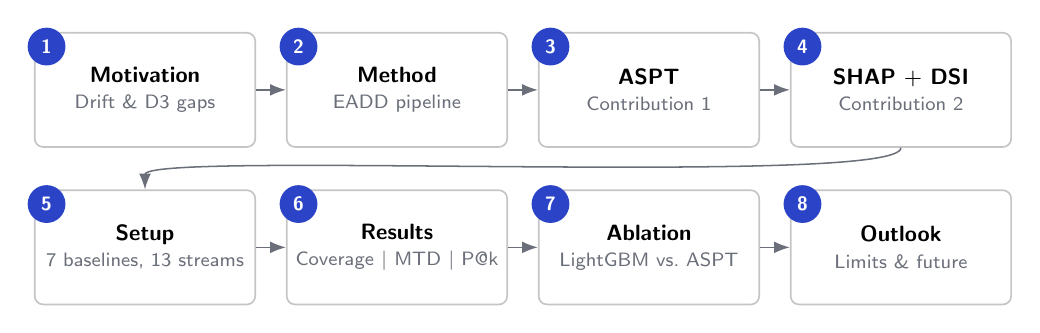
\begin{tikzpicture}[font=\footnotesize,
    stepbox/.style={draw=ink!25,fill=white,line width=0.6pt,rounded corners=3pt,
                  minimum width=2.8cm,minimum height=1.45cm,align=center,inner sep=3pt},
    num/.style={circle,fill=cobalt,text=white,font=\scriptsize\bfseries,
                inner sep=0pt,minimum size=4.8mm},
    arr/.style={-{Latex[length=2mm]},graphite,line width=0.55pt}]
  \node[stepbox] (s1) at (0,0)    {\textbf{Motivation}\\{\scriptsize\color{graphite}Drift \& D3 gaps}};
  \node[stepbox] (s2) at (3.2,0)  {\textbf{Method}\\{\scriptsize\color{graphite}EADD pipeline}};
  \node[stepbox] (s3) at (6.4,0)  {\textbf{ASPT}\\{\scriptsize\color{graphite}Contribution 1}};
  \node[stepbox] (s4) at (9.6,0)  {\textbf{SHAP $+$ DSI}\\{\scriptsize\color{graphite}Contribution 2}};
  \node[stepbox] (s5) at (0,-2)   {\textbf{Setup}\\{\scriptsize\color{graphite}7 baselines, 13 streams}};
  \node[stepbox] (s6) at (3.2,-2) {\textbf{Results}\\{\scriptsize\color{graphite}Coverage \textbar{} MTD \textbar{} P@k}};
  \node[stepbox] (s7) at (6.4,-2) {\textbf{Ablation}\\{\scriptsize\color{graphite}LightGBM vs.\ ASPT}};
  \node[stepbox] (s8) at (9.6,-2) {\textbf{Outlook}\\{\scriptsize\color{graphite}Limits \& future}};
  \foreach \i/\n in {s1/1,s2/2,s3/3,s4/4,s5/5,s6/6,s7/7,s8/8}
    \node[num] at ([xshift=-1.25cm,yshift=0.55cm]\i.center) {\n};
  \draw[arr] (s1) -- (s2); \draw[arr] (s2) -- (s3); \draw[arr] (s3) -- (s4);
  \draw[arr] (s4.south) .. controls ([yshift=-0.5cm]s4.south) and ([yshift=0.5cm]s5.north) .. (s5.north);
  \draw[arr] (s5) -- (s6); \draw[arr] (s6) -- (s7); \draw[arr] (s7) -- (s8);
\end{tikzpicture}

\vspace{1.0em}
\centering\small\color{graphite}
EADD answers \textcolor{cobalt}{\textbf{whether}}, \textcolor{cobalt}{\textbf{when}},
\textcolor{cobalt}{\textbf{which}}, and \textcolor{cobalt}{\textbf{how severe}}\,---\,in one pipeline.
\end{frame}

% ════════════════════ SECTION 1 ════════════════════
\sectionDivider{01}{The Problem}{Why production ML detectors miss the mark}

\setsec{01 \textbar{} THE PROBLEM}
\begin{frame}{Production ML models fail silently}
\vspace{0.2em}
\begin{columns}[T,onlytextwidth]
\column{0.55\textwidth}
\centering
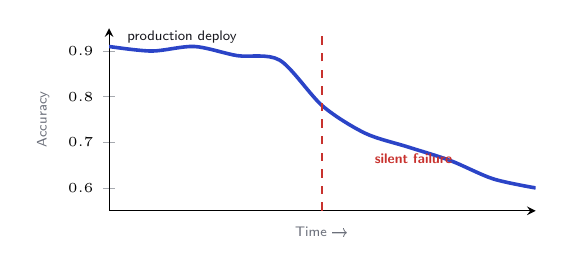
\begin{tikzpicture}[font=\scriptsize]
  \begin{axis}[
    width=7.0cm,height=3.9cm,
    axis lines=left,
    xlabel={Time \textrightarrow{}}, ylabel={Accuracy},
    ymin=0.55,ymax=0.95,xmin=0,xmax=10,
    xtick=\empty, ytick={0.6,0.7,0.8,0.9},
    yticklabel style={font=\tiny},
    xlabel style={font=\tiny,text=graphite},
    ylabel style={font=\tiny,text=graphite},
    tick style={graphite!60}, every axis line/.style={graphite!60},
  ]
    \addplot[cobalt,line width=1.3pt,smooth] coordinates
      {(0,0.91)(1,0.90)(2,0.91)(3,0.89)(4,0.88)(5,0.78)(6,0.72)(7,0.69)(8,0.66)(9,0.62)(10,0.60)};
    \draw[crimson,dashed,line width=0.8pt] (axis cs:5,0.55) -- (axis cs:5,0.95);
    \node[text=crimson,font=\tiny\bfseries,anchor=south] at (axis cs:5,0.95) {drift onset};
    \node[text=ink,font=\tiny,anchor=west] at (axis cs:0.2,0.93) {production deploy};
    \node[text=crimson,font=\tiny\bfseries,anchor=west] at (axis cs:6,0.665) {silent failure};
  \end{axis}
\end{tikzpicture}

\smallskip
{\footnotesize \textbf{Distribution drift} silently degrades models.
Existing detectors raise a \emph{binary} alarm; practitioners need more:}

\smallskip

\begin{tikzpicture}[font=\footnotesize,
   q/.style={draw=cobalt,fill=cobalt!8,line width=0.5pt,rounded corners=2pt,
             inner xsep=3pt,inner ysep=2.5pt,text=cobalt,font=\scriptsize\bfseries}]
  \node[q] (q1) {Which features?};
  \node[q,right=1.4mm of q1] (q2) {How severe?};
  \node[q,right=1.4mm of q2] (q3) {Real or noise?};
\end{tikzpicture}

\column{0.45\textwidth}
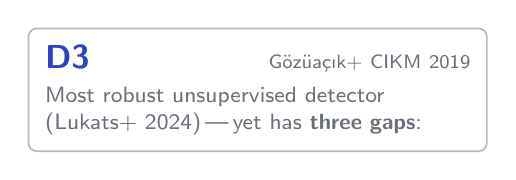
\begin{tikzpicture}
  \node[draw=ink!30,fill=white,line width=0.6pt,rounded corners=3pt,
        inner sep=6pt,text width=5.4cm,align=left,font=\footnotesize] (card) {%
    \textbf{\color{cobalt}\large D3} \hfill {\scriptsize\color{graphite}Gözüaçık+ CIKM 2019}\\[3pt]
    {\color{graphite}Most robust unsupervised detector
     (Lukats+ 2024)\,---\,yet has \textbf{three gaps}:}
  };
\end{tikzpicture}

\vspace{0.3em}
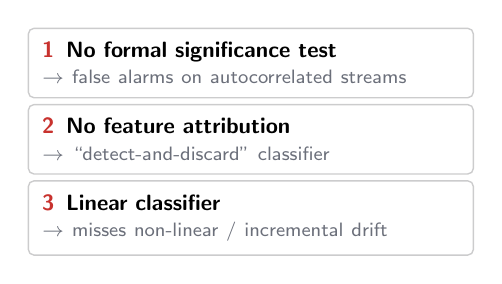
\begin{tikzpicture}[font=\footnotesize,
   gap/.style={draw=ink!22,fill=white,line width=0.5pt,rounded corners=2pt,
               text width=5.3cm,align=left,inner sep=5pt}]
  \node[gap] (g1) {%
    {\color{crimson}\textbf{1}}\enspace \textbf{No formal significance test}\\
    {\scriptsize\color{graphite}$\to$ false alarms on autocorrelated streams}};
  \node[gap,below=2pt of g1] (g2) {%
    {\color{crimson}\textbf{2}}\enspace \textbf{No feature attribution}\\
    {\scriptsize\color{graphite}$\to$ ``detect-and-discard'' classifier}};
  \node[gap,below=2pt of g2] (g3) {%
    {\color{crimson}\textbf{3}}\enspace \textbf{Linear classifier}\\
    {\scriptsize\color{graphite}$\to$ misses non-linear / incremental drift}};
\end{tikzpicture}
\end{columns}
\end{frame}

% ──────────────────── CAPABILITY MATRIX ────────────────────
\begin{frame}{Capability matrix \textbar{} the integration gap}
\vspace{0.2em}
\centering

\begin{tikzpicture}[font=\footnotesize,
    qcard/.style={draw,line width=0.8pt,rounded corners=3pt,
                  minimum width=3.6cm,minimum height=1.1cm,align=center,inner sep=4pt}]
  \node[qcard,draw=cobalt,fill=cobalt!8]  (q1) at (-5.4,0)
    {\textbf{\color{cobalt}WHETHER}\\{\scriptsize\color{graphite}Binary drift alarm}};
  \node[qcard,draw=emerald,fill=emerald!8] (q2) at (0,0)
    {\textbf{\color{emerald}WHICH}\\{\scriptsize\color{graphite}Feature attribution}};
  \node[qcard,draw=gold!85!black,fill=gold!18] (q3) at (5.4,0)
    {\textbf{\color{gold!70!black}HOW SEVERE}\\{\scriptsize\color{graphite}Severity quantification}};
\end{tikzpicture}

\vspace{0.5em}
\centering
\renewcommand{\arraystretch}{1.25}
\setlength{\tabcolsep}{8pt}
{\footnotesize
\begin{tabular}{@{}>{\raggedright\arraybackslash}p{3.6cm} c c c c@{}}
\toprule
\rowcolor{ink!90}
\textcolor{white}{\textbf{Approach}} & \textcolor{white}{\textbf{Whether}} &
\textcolor{white}{\textbf{Which}}    & \textcolor{white}{\textbf{Severity}}  &
\textcolor{white}{\textbf{Streaming}} \\
\midrule
DDM / EDDM          & {\color{emerald}$\checkmark$} & {\color{crimson}$\times$} & {\color{crimson}$\times$} & {\color{emerald}$\checkmark$} \\
KS / KSWIN          & {\color{emerald}$\checkmark$} & {\color{gold!70!black}$\sim$} & {\color{crimson}$\times$} & {\color{emerald}$\checkmark$} \\
D3                  & {\color{emerald}$\checkmark$} & {\color{crimson}$\times$} & {\color{crimson}$\times$} & {\color{emerald}$\checkmark$} \\
Vertex AI / Clarify & {\color{emerald}$\checkmark$} & {\color{emerald}$\checkmark$} & {\color{gold!70!black}$\sim$} & {\color{crimson}$\times$} \\
TRIPODD / HDPD      & {\color{emerald}$\checkmark$} & {\color{emerald}$\checkmark$} & {\color{crimson}$\times$} & {\color{crimson}$\times$} \\
\midrule
\rowcolor{cobalt!88}
\textcolor{white}{\textbf{EADD (this work)}} &
\textcolor{white}{$\checkmark$} & \textcolor{white}{$\checkmark$} &
\textcolor{white}{$\checkmark$} & \textcolor{white}{$\checkmark$} \\
\bottomrule
\end{tabular}}

\vspace{0.6em}
{\scriptsize\color{graphite}\itshape No prior unsupervised streaming detector integrates \emph{whether} $+$ \emph{which} $+$ \emph{severity}.}
\end{frame}

% ──────────────────── CONTRIBUTIONS ────────────────────
\begin{frame}{Three contributions, one pipeline}
\vspace{0.3em}
\centering
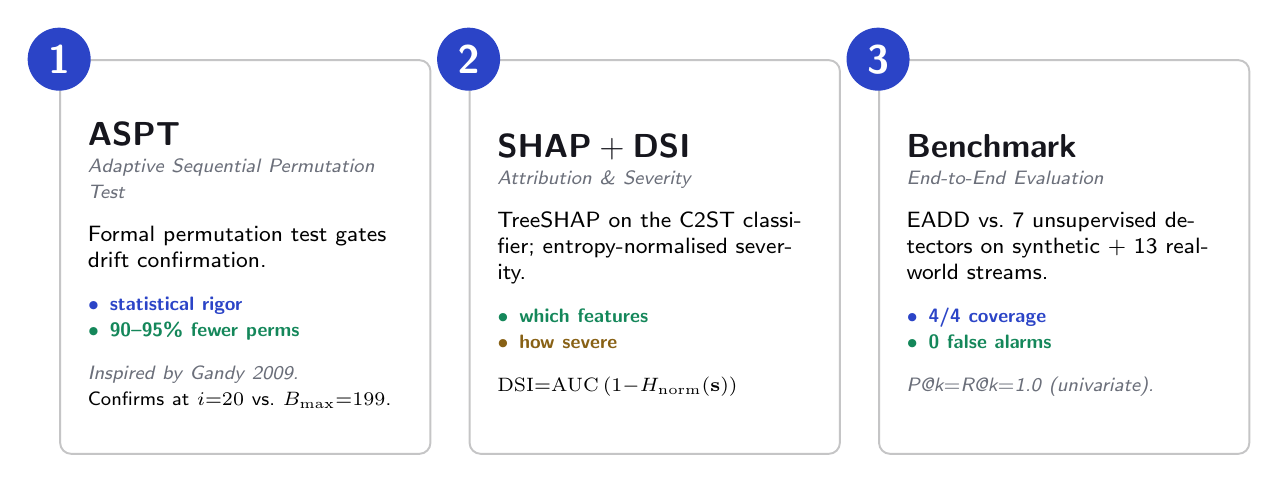
\begin{tikzpicture}[font=\footnotesize,
    card/.style={draw=ink!25,line width=0.7pt,rounded corners=4pt,
                 fill=white,minimum width=4.5cm,minimum height=5.0cm,
                 inner sep=10pt,align=left,text width=4.0cm,anchor=center},
    badge/.style={circle,fill=cobalt,text=white,font=\Large\bfseries,
                  inner sep=0pt,minimum size=8mm}]
  \node[card] (c1) at (-5.2,0) {%
    \vspace{0.6em}\\
    \textbf{\color{ink}\large ASPT}\\
    {\scriptsize\itshape\color{graphite}Adaptive Sequential Permutation Test}\\[6pt]
    Formal permutation test gates drift confirmation.\\[6pt]
    {\scriptsize\color{cobalt}\textbf{$\bullet$\enspace statistical rigor}}\\
    {\scriptsize\color{emerald}\textbf{$\bullet$\enspace 90--95\% fewer perms}}\\[6pt]
    {\scriptsize\color{graphite}\itshape Inspired by Gandy 2009.}\\
    {\scriptsize Confirms at $i{=}20$ vs.\ $B_{\max}{=}199$.}};
  \node[card] (c2) at (0,0) {%
    \vspace{0.6em}\\
    \textbf{\color{ink}\large SHAP $+$ DSI}\\
    {\scriptsize\itshape\color{graphite}Attribution \& Severity}\\[6pt]
    TreeSHAP on the C2ST classifier; entropy-normalised severity.\\[6pt]
    {\scriptsize\color{emerald}\textbf{$\bullet$\enspace which features}}\\
    {\scriptsize\color{gold!70!black}\textbf{$\bullet$\enspace how severe}}\\[6pt]
    {\scriptsize $\mathrm{DSI}{=}\mathrm{AUC}\,(1{-}H_{\mathrm{norm}}(\mathbf{s}))$}};
  \node[card] (c3) at (5.2,0) {%
    \vspace{0.6em}\\
    \textbf{\color{ink}\large Benchmark}\\
    {\scriptsize\itshape\color{graphite}End-to-End Evaluation}\\[6pt]
    EADD vs.\ 7 unsupervised detectors on synthetic $+$ 13 real-world streams.\\[6pt]
    {\scriptsize\color{cobalt}\textbf{$\bullet$\enspace 4/4 coverage}}\\
    {\scriptsize\color{emerald}\textbf{$\bullet$\enspace 0 false alarms}}\\[6pt]
    {\scriptsize\color{graphite}\itshape P@k$=$R@k$=$1.0 (univariate).}};
  \node[badge] at (c1.north west) {1};
  \node[badge] at (c2.north west) {2};
  \node[badge] at (c3.north west) {3};
\end{tikzpicture}
\end{frame}

% ════════════════════ SECTION 2 ════════════════════
\sectionDivider{02}{The EADD Pipeline}{Four-step streaming detector}

\setsec{02 \textbar{} THE EADD PIPELINE}
\begin{frame}{End-to-end detection pipeline}
\vspace{-0.4em}
\centering
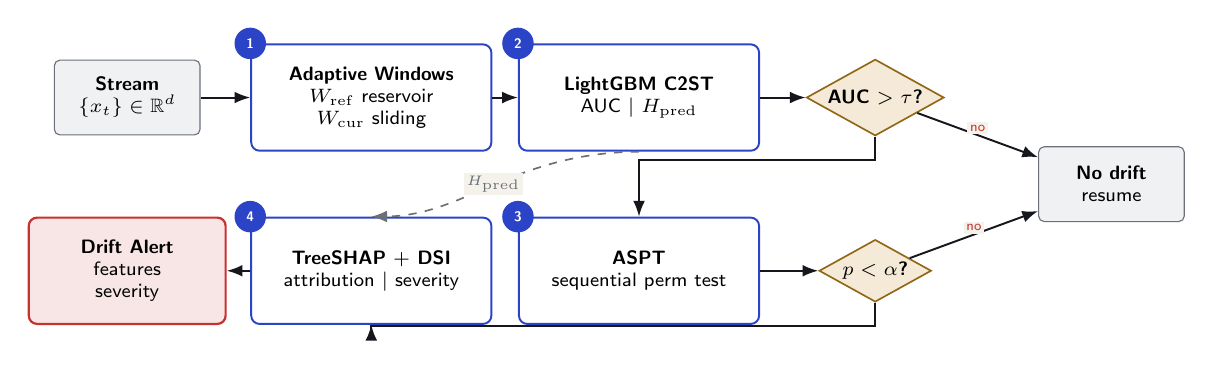
\begin{tikzpicture}[font=\scriptsize,
    proc/.style={draw=cobalt,fill=white,line width=0.7pt,rounded corners=3pt,
                 minimum width=3.05cm,minimum height=1.35cm,align=center,inner sep=3pt},
    dec/.style={diamond,draw=gold!75!black,fill=gold!18,line width=0.6pt,
                aspect=1.8,align=center,inner sep=1pt,font=\scriptsize\bfseries},
    term/.style={draw=graphite,fill=graphite!10,rounded corners=2pt,align=center,
                  minimum width=1.85cm,minimum height=0.95cm},
    alert/.style={draw=crimson,fill=crimson!12,line width=0.8pt,rounded corners=3pt,
                  align=center,minimum width=2.5cm,minimum height=1.35cm},
    arr/.style={-{Latex[length=2mm]},ink,line width=0.7pt},
    darr/.style={-{Latex[length=2mm]},graphite,line width=0.6pt,dashed},
    num/.style={circle,fill=cobalt,text=white,font=\tiny\bfseries,
                inner sep=0pt,minimum size=4mm}]
  \node[term] (in) at (-6.5,0) {\textbf{Stream}\\$\{x_t\}\in\mathbb{R}^d$};
  \node[proc] (s1) at (-3.4,0) {\textbf{Adaptive Windows}\\$W_\mathrm{ref}$ reservoir\\$W_\mathrm{cur}$ sliding};
  \node[proc] (s2) at (0,0)    {\textbf{LightGBM C2ST}\\AUC \textbar{} $H_\mathrm{pred}$};
  \node[dec]  (d1) at (3.0,0)  {AUC $> \tau$?};
  \node[proc] (s3) at (0,-2.2) {\textbf{ASPT}\\sequential perm test};
  \node[dec]  (d2) at (3.0,-2.2) {$p < \alpha$?};
  \node[proc] (s4) at (-3.4,-2.2) {\textbf{TreeSHAP $+$ DSI}\\attribution \textbar{} severity};
  \node[alert] (out) at (-6.5,-2.2) {\textbf{Drift Alert}\\\scriptsize features\\\scriptsize severity};
  \node[term] (nd) at (6.0,-1.1) {\textbf{No drift}\\resume};
  \node[num] at (s1.north west) {1};
  \node[num] at (s2.north west) {2};
  \node[num] at (s3.north west) {3};
  \node[num] at (s4.north west) {4};
  \draw[arr] (in) -- (s1);
  \draw[arr] (s1) -- (s2);
  \draw[arr] (s2) -- (d1);
  \draw[arr] (d1) -- node[above,font=\tiny,text=crimson,fill=paper,inner sep=1pt] {no} (nd);
  \draw[arr] (d1.south) -- ++(0,-0.3) -| (s3.north);
  \draw[arr] (s3) -- (d2);
  \draw[arr] (d2) -- node[above,font=\tiny,text=crimson,fill=paper,inner sep=1pt] {no} (nd);
  \draw[arr] (d2.south) -- ++(0,-0.3) -| (s4.south);
  \draw[arr] (s4) -- (out);
  \draw[darr] (s2.south) .. controls (-1.6,-0.7) and (-2.2,-1.5) .. (s4.north)
    node[midway,fill=paper,font=\tiny,text=graphite,inner sep=1pt] {$H_\mathrm{pred}$};
\end{tikzpicture}

\vspace{0.5em}
\centering{\footnotesize\color{graphite}\itshape
Two-stage gate $\Rightarrow$ Type I error bound:
$\Pr(\mathrm{AUC}{>}\tau\mid H_0)\cdot\alpha \leq \alpha$.}
\end{frame}

% ════════════════════ ASPT ════════════════════
\setsec{02 \textbar{} CONTRIBUTION 1}
\begin{frame}{ASPT\,---\,Adaptive Sequential Permutation Test}
\begin{columns}[T,onlytextwidth]
\column{0.50\textwidth}
\textbf{Problem.} D3's fixed AUC threshold $\to$ false alarms on autocorrelated streams.

\smallskip
\textbf{Idea.} Permute labels iteratively; stop early once evidence is decisive.

\smallskip
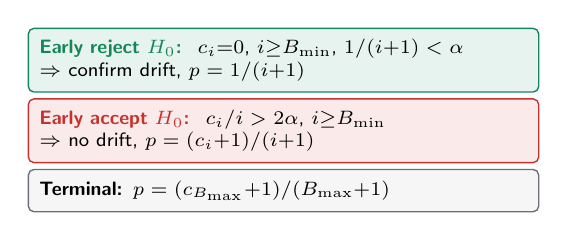
\begin{tikzpicture}[font=\scriptsize,
    box/.style={draw=ink!30,line width=0.5pt,rounded corners=2pt,
                fill=white,text width=6.2cm,inner sep=4pt,align=left}]
  \node[box,draw=emerald,fill=emerald!10] (r) {%
    \textbf{\color{emerald}Early reject $H_0$:}\;
    $c_i{=}0$, $i{\ge}B_{\min}$, $1/(i{+}1)<\alpha$\\
    $\Rightarrow$ confirm drift, $p=1/(i{+}1)$};
  \node[box,draw=crimson,fill=crimson!10,below=2pt of r] (a) {%
    \textbf{\color{crimson}Early accept $H_0$:}\;
    $c_i/i > 2\alpha$, $i{\ge}B_{\min}$\\
    $\Rightarrow$ no drift, $p=(c_i{+}1)/(i{+}1)$};
  \node[box,draw=graphite,fill=graphite!6,below=2pt of a] (t) {%
    \textbf{Terminal:} $p=(c_{B_{\max}}{+}1)/(B_{\max}{+}1)$};
\end{tikzpicture}

\column{0.50\textwidth}
\centering
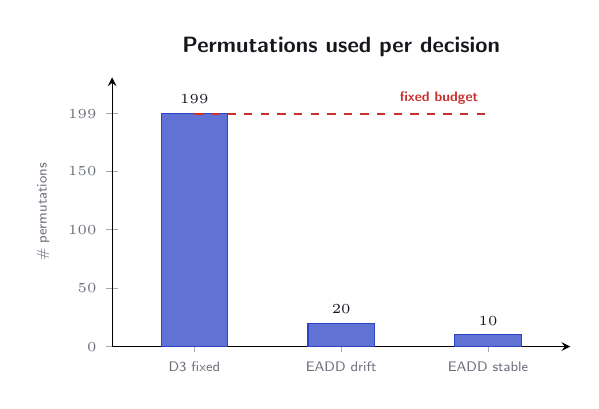
\begin{tikzpicture}[font=\tiny]
  \begin{axis}[
    width=7.4cm,height=5.0cm,
    title={\footnotesize\color{ink}\textbf{Permutations used per decision}},
    title style={yshift=-2pt},
    ylabel={\#~permutations}, ymin=0,ymax=230,
    symbolic x coords={D3 fixed,EADD drift,EADD stable},
    xtick=data, ytick={0,50,100,150,199},
    ybar,bar width=24pt,
    nodes near coords,
    nodes near coords style={font=\tiny\bfseries,text=ink},
    axis lines=left,
    every tick label/.style={font=\tiny,text=graphite},
    ylabel style={font=\tiny,text=graphite},
    tick style={graphite!60}, every axis line/.style={graphite!60},
    enlarge x limits=0.28,
  ]
    \addplot[fill=cobalt!75,draw=cobalt]
      coordinates {(D3 fixed,199) (EADD drift,20) (EADD stable,10)};
    \draw[crimson,line width=0.7pt,dashed]
      (axis cs:D3 fixed,199) -- (axis cs:EADD stable,199);
    \node[text=crimson,font=\tiny\bfseries,anchor=south east]
      at (axis cs:EADD stable,199) {fixed budget};
  \end{axis}
\end{tikzpicture}

\vspace{0.2em}
\colorbox{cobalt!16}{\small\textbf{\color{ink}90--95\% fewer permutations}
\textbar{} $\alpha$ preserved}
\end{columns}
\end{frame}

% ════════════════════ SHAP + DSI ════════════════════
\setsec{02 \textbar{} CONTRIBUTION 2}
\begin{frame}{SHAP attribution $+$ Drift Severity Index}
\begin{columns}[T,onlytextwidth]
\column{0.48\textwidth}
\textbf{TreeSHAP on the C2ST classifier} (which D3 discards).

\smallskip
\[
\bar\phi_j = \tfrac{1}{n}\sum_i |\phi_j^{(i)}|, \quad
s_j = \bar\phi_j \,/\, \textstyle\sum_k \bar\phi_k
\]
{\scriptsize\color{graphite}Normalised attribution share $\to$ which features drifted.}

\smallskip
\textbf{Drift Severity Index.}
\[
\boxed{\;\mathrm{DSI}=\mathrm{AUC}\times(1-H_{\mathrm{norm}}(\mathbf{s}))\;}
\]
{\scriptsize $H_{\mathrm{norm}}(\mathbf{s})=-\sum_j s_j\log_2 s_j\,/\,\log_2 d \in[0,1]$\,---\,dimensionality-invariant.}

\column{0.52\textwidth}
\centering\textbf{\small Severity gradient \& prescription tiers}

\vspace{0.3em}
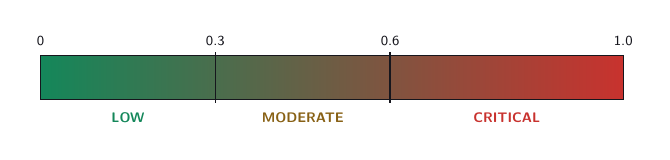
\begin{tikzpicture}[font=\scriptsize]
  \shade[left color=emerald,middle color=gold,right color=crimson]
    (0,0) rectangle (7.4,0.55);
  \draw[ink,line width=0.4pt] (0,0) rectangle (7.4,0.55);
  \draw[ink,line width=0.5pt] (2.22,-0.05) -- (2.22,0.60);
  \draw[ink,line width=0.5pt] (4.44,-0.05) -- (4.44,0.60);
  \node[anchor=north,font=\tiny\bfseries,text=emerald] at (1.11,-0.05) {LOW};
  \node[anchor=north,font=\tiny\bfseries,text=gold!70!black] at (3.33,-0.05) {MODERATE};
  \node[anchor=north,font=\tiny\bfseries,text=crimson] at (5.92,-0.05) {CRITICAL};
  \node[anchor=south,font=\tiny,text=ink] at (0,0.55) {0};
  \node[anchor=south,font=\tiny,text=ink] at (2.22,0.55) {0.3};
  \node[anchor=south,font=\tiny,text=ink] at (4.44,0.55) {0.6};
  \node[anchor=south,font=\tiny,text=ink] at (7.4,0.55) {1.0};
\end{tikzpicture}

\vspace{1.2em}
{\footnotesize
\begin{tabular}{@{}l p{4.6cm}@{}}
\toprule
\textbf{Tier} & \textbf{Recommended action} \\
\midrule
\textcolor{emerald}{\textbf{Low}} ($<\!0.3$)        & Diffuse shift $\to$ scheduled retrain \\
\textcolor{gold!70!black}{\textbf{Moderate}} (0.3--0.6) & Subset drift $\to$ audit shared source \\
\textcolor{crimson}{\textbf{Critical}} ($>\!0.6$)           & Concentrated $\to$ audit pipeline \\
\bottomrule
\end{tabular}}

\vspace{0.2em}
{\scriptsize\itshape\color{graphite}Heuristic tiers; require domain calibration.}
\end{columns}
\end{frame}

% ════════════════════ SECTION 3 ════════════════════
\sectionDivider{03}{Experiments \& Results}{What does EADD actually do?}

\setsec{03 \textbar{} EXPERIMENTS}
\begin{frame}{Experimental setup}
\centering
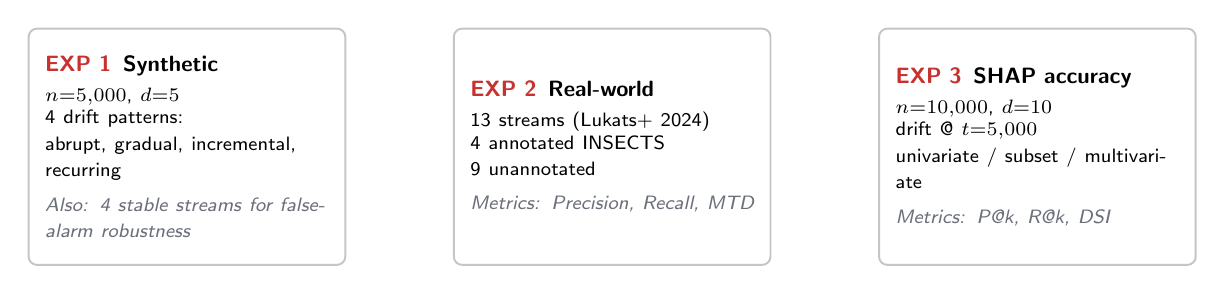
\begin{tikzpicture}[font=\footnotesize,
    card/.style={draw=ink!25,line width=0.7pt,rounded corners=3pt,
                 fill=white,minimum width=4.0cm,minimum height=3.0cm,
                 inner sep=6pt,align=left,text width=3.6cm}]
  \node[card] (e1) at (-5.4,0) {
    {\fontsize{8}{10}\selectfont\color{crimson}\textbf{EXP 1}}\enspace\textbf{Synthetic}\\[3pt]
    {\scriptsize $n{=}5{,}000$, $d{=}5$\\
    4 drift patterns:\\abrupt, gradual, incremental, recurring}\\[3pt]
    {\scriptsize\color{graphite}\itshape Also: 4 stable streams for false-alarm robustness}
  };
  \node[card] (e2) at (0,0) {
    {\fontsize{8}{10}\selectfont\color{crimson}\textbf{EXP 2}}\enspace\textbf{Real-world}\\[3pt]
    {\scriptsize 13 streams (Lukats+ 2024)\\
    4 annotated INSECTS\\9 unannotated}\\[3pt]
    {\scriptsize\color{graphite}\itshape Metrics: Precision, Recall, MTD}
  };
  \node[card] (e3) at (5.4,0) {
    {\fontsize{8}{10}\selectfont\color{crimson}\textbf{EXP 3}}\enspace\textbf{SHAP accuracy}\\[3pt]
    {\scriptsize $n{=}10{,}000$, $d{=}10$\\
    drift @ $t{=}5{,}000$\\univariate / subset / multivariate}\\[3pt]
    {\scriptsize\color{graphite}\itshape Metrics: P@k, R@k, DSI}
  };
\end{tikzpicture}

\vspace{0.6em}
\centering
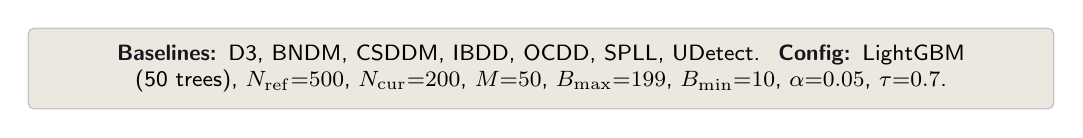
\begin{tikzpicture}[font=\footnotesize]
  \node[draw=ink!25,line width=0.5pt,rounded corners=2pt,fill=mist,
        inner sep=6pt,text width=12.6cm,align=center] {%
    \textbf{\color{ink}Baselines:} D3, BNDM, CSDDM, IBDD, OCDD, SPLL, UDetect.\;
    \textbf{\color{ink}Config:} LightGBM (50 trees),
    $N_\mathrm{ref}{=}500$, $N_\mathrm{cur}{=}200$, $M{=}50$,
    $B_{\max}{=}199$, $B_{\min}{=}10$, $\alpha{=}0.05$, $\tau{=}0.7$.};
\end{tikzpicture}
\end{frame}

% ──────────────────── HEADLINE STATS ────────────────────
\setsec{03 \textbar{} HEADLINE}
\begin{frame}{Headline results}
\vspace{0.4em}
\centering
\statTile{4/4}{synthetic\\coverage}{cobalt}\hfill
\statTile{0}{false alarms\\on stable streams}{emerald}\hfill
\statTile{8$\boldsymbol{\times}$}{faster MTD\\vs.\ D3 (incremental)}{crimson}\hfill
\statTile{1.00}{P@k$=$R@k\\(univariate SHAP)}{gold!75!black}

\vspace{1.0em}
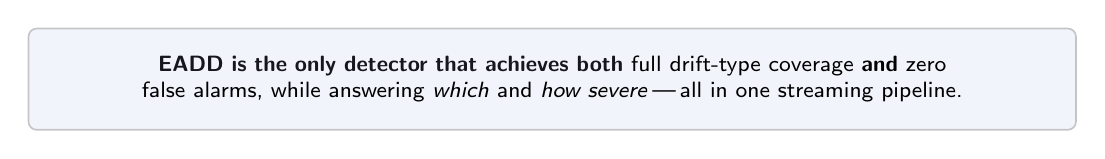
\begin{tikzpicture}[font=\footnotesize]
  \node[draw=ink!25,line width=0.6pt,rounded corners=3pt,fill=cobalt!6,
        inner sep=10pt,text width=12.6cm,align=center] {%
    \textbf{\color{ink}EADD is the only detector that achieves both}
    full drift-type coverage \textbf{and} zero false alarms,
    while answering \textit{which} and \textit{how severe}\,---\,all in one streaming pipeline.};
\end{tikzpicture}

\vspace{0.6em}
{\scriptsize\color{graphite}Mann--Whitney U vs.\ D3 on autocorrelated streams: $p=0.0101$ ($\tau{=}0.6$).}
\end{frame}

% ──────────────────── RESULT 1 ────────────────────
\setsec{03 \textbar{} RESULT 1}
\begin{frame}{Synthetic coverage vs.\ false alarms}
\centering
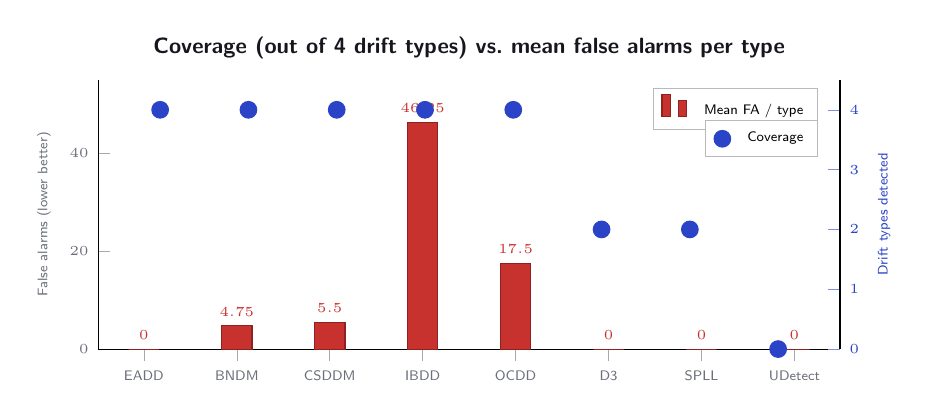
\begin{tikzpicture}[font=\tiny]
  \begin{axis}[
    width=11.0cm,height=5.0cm,
    title={\footnotesize\color{ink}\textbf{Coverage (out of 4 drift types) vs.\ mean false alarms per type}},
    title style={yshift=-2pt},
    ybar,bar width=11pt, ymin=0,ymax=55,
    enlarge x limits=0.07,
    symbolic x coords={EADD,BNDM,CSDDM,IBDD,OCDD,D3,SPLL,UDetect},
    xtick=data, ylabel={False alarms (lower better)},
    axis y line*=left, axis x line*=bottom,
    every axis label/.style={font=\tiny,text=graphite},
    every tick label/.style={font=\tiny,text=graphite},
    tick style={graphite!60}, every axis line/.style={graphite!60},
    nodes near coords, nodes near coords style={font=\tiny\bfseries,text=crimson},
    nodes near coords align={vertical},
    legend style={at={(0.97,0.97)},anchor=north east,font=\tiny,
                  draw=ink!30,fill=white,column sep=4pt},
  ]
    \addplot[fill=crimson,draw=crimson!70!black]
      coordinates {(EADD,0.00) (BNDM,4.75) (CSDDM,5.50) (IBDD,46.25)
                   (OCDD,17.50) (D3,0.00) (SPLL,0.00) (UDetect,0)};
    \addlegendentry{Mean FA / type};
  \end{axis}
  \begin{axis}[
    width=11.0cm,height=5.0cm,
    ymin=0,ymax=4.5,ytick={0,1,2,3,4},
    ylabel={Drift types detected},
    axis y line*=right, axis x line=none,
    symbolic x coords={EADD,BNDM,CSDDM,IBDD,OCDD,D3,SPLL,UDetect},
    every axis label/.style={font=\tiny,text=cobalt},
    every tick label/.style={font=\tiny,text=cobalt},
    tick style={cobalt!60}, every axis line/.style={cobalt!60},
    legend style={at={(0.97,0.85)},anchor=north east,font=\tiny,
                  draw=ink!30,fill=white,column sep=4pt},
  ]
    \addplot[only marks,mark=*,mark size=3pt,cobalt]
      coordinates {(EADD,4) (BNDM,4) (CSDDM,4) (IBDD,4)
                   (OCDD,4) (D3,2) (SPLL,2) (UDetect,0)};
    \addlegendentry{Coverage};
  \end{axis}
\end{tikzpicture}

\vspace{0.2em}

\begin{tikzpicture}[font=\footnotesize]
\node[fill=cobalt,rounded corners=3pt,text=white,inner sep=5pt,
      text width=12.6cm,align=center] {%
EADD: \textbf{4/4 coverage} AND \textbf{0 false alarms.}
BNDM/CSDDM/IBDD/OCDD also hit 4/4 but pay heavy FA cost;
D3/SPLL keep 0 FA only by missing half the drift types.};
\end{tikzpicture}
\end{frame}

% ──────────────────── RESULT 2 ────────────────────
\setsec{03 \textbar{} RESULT 2}
\begin{frame}{INSECTS\,---\,faster detection on incremental drift}
\centering
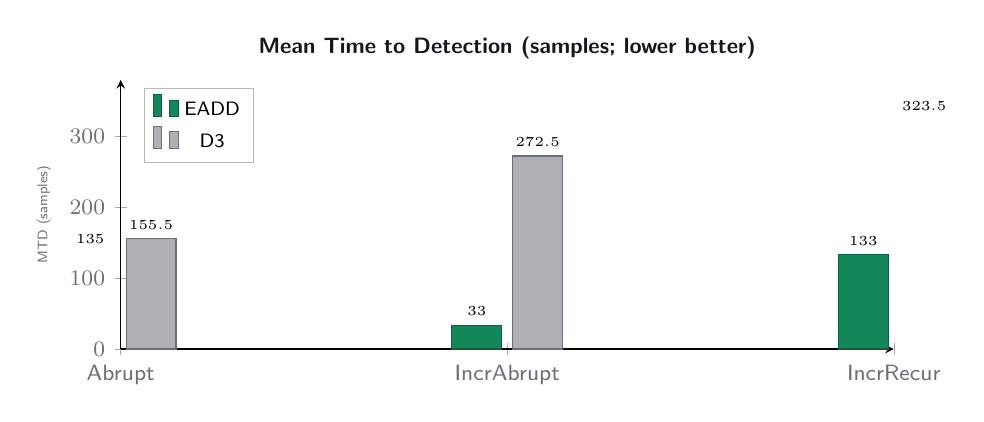
\begin{tikzpicture}[font=\tiny]
  \begin{axis}[
    width=11.4cm,height=5.0cm,
    title={\footnotesize\color{ink}\textbf{Mean Time to Detection (samples; lower better)}},
    title style={yshift=-2pt},
    ybar=4pt,bar width=18pt, ymin=0,ymax=380,
    enlarge x limits=0.25,
    symbolic x coords={Abrupt,IncrAbrupt,IncrRecur},
    xtick=data, ylabel={MTD (samples)},
    axis lines=left,
    every axis label/.style={font=\tiny,text=graphite},
    every tick label/.style={font=\footnotesize,text=graphite},
    tick style={graphite!60}, every axis line/.style={graphite!60},
    nodes near coords, nodes near coords style={font=\tiny\bfseries},
    legend style={at={(0.03,0.97)},anchor=north west,legend columns=1,
                  font=\scriptsize,draw=ink!30,fill=white},
  ]
    \addplot[fill=emerald,draw=emerald!70!black]
      coordinates {(Abrupt,135) (IncrAbrupt,33) (IncrRecur,133)};
    \addplot[fill=graphite!55,draw=graphite]
      coordinates {(Abrupt,155.5) (IncrAbrupt,272.5) (IncrRecur,323.5)};
    \legend{EADD,D3}
  \end{axis}
\end{tikzpicture}

\vspace{0.2em}
\centering
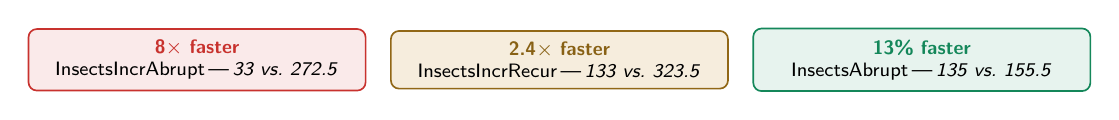
\begin{tikzpicture}[font=\scriptsize,
   tile/.style={rounded corners=3pt,line width=0.6pt,inner sep=4pt,
                text width=4.0cm,align=center}]
  \node[tile,draw=crimson,fill=crimson!10] (a)
    {\textbf{\color{crimson}8$\times$ faster}\\InsectsIncrAbrupt\,---\,\textit{33 vs.\ 272.5}};
  \node[tile,draw=gold!75!black,fill=gold!15,right=0.3cm of a] (b)
    {\textbf{\color{gold!70!black}2.4$\times$ faster}\\InsectsIncrRecur\,---\,\textit{133 vs.\ 323.5}};
  \node[tile,draw=emerald,fill=emerald!10,right=0.3cm of b] (c)
    {\textbf{\color{emerald}13\% faster}\\InsectsAbrupt\,---\,\textit{135 vs.\ 155.5}};
\end{tikzpicture}

\vspace{0.3em}
{\scriptsize\color{graphite}\itshape EADD beats D3 on MTD in all three jointly detected INSECTS streams; InsectsGradual missed by both.}
\end{frame}

% ──────────────────── RESULT 3 ────────────────────
\setsec{03 \textbar{} RESULT 3}
\begin{frame}{SHAP attribution\,---\,P@k $=$ R@k $=$ 1.0}
\begin{columns}[T,onlytextwidth]
\column{0.55\textwidth}
\centering
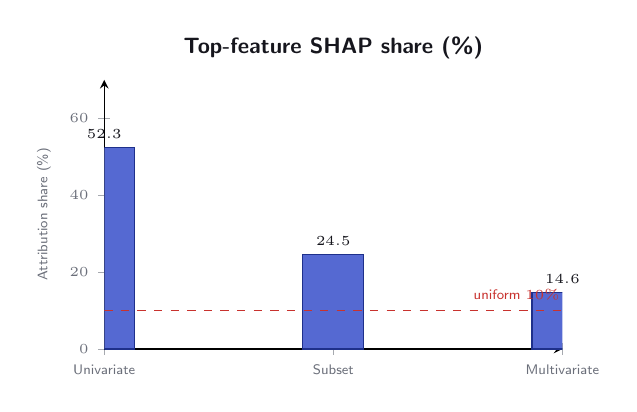
\begin{tikzpicture}[font=\tiny]
  \begin{axis}[
    width=7.4cm,height=5.0cm,
    title={\footnotesize\color{ink}\textbf{Top-feature SHAP share (\%)}},
    title style={yshift=-2pt},
    ybar,bar width=22pt, ymin=0,ymax=70,
    enlarge x limits=0.22,
    symbolic x coords={Univariate,Subset,Multivariate},
    xtick=data, ylabel={Attribution share (\%)},
    axis lines=left,
    every axis label/.style={font=\tiny,text=graphite},
    every tick label/.style={font=\tiny,text=graphite},
    tick style={graphite!60}, every axis line/.style={graphite!60},
    nodes near coords, nodes near coords style={font=\tiny\bfseries,text=ink},
  ]
    \addplot[fill=cobalt!80,draw=cobalt!70!black]
      coordinates {(Univariate,52.3) (Subset,24.5) (Multivariate,14.6)};
    \draw[crimson,dashed,line width=0.6pt]
      (axis cs:Univariate,10) -- (axis cs:Multivariate,10)
      node[pos=0.9,above,font=\tiny,text=crimson] {uniform $10\%$};
  \end{axis}
\end{tikzpicture}

\column{0.45\textwidth}
\centering
\textbf{\small Perfect attribution \textbar{} P@k $=$ R@k $=$ 1.0}

\vspace{0.3em}
\setlength{\tabcolsep}{4pt}
{\footnotesize
\begin{tabular}{@{}l c c c@{}}
\toprule
\textbf{Scenario} & \textbf{AUC} & \textbf{Top feat.} & \textbf{DSI} \\
\midrule
Univariate (1/10)    & 0.784 & \textbf{F3} (52.3\%) & 0.193 \\
Subset (3/10)        & 0.809 & F5 (24.5\%)          & 0.096 \\
Multivariate (10/10) & 0.806 & F2 (14.6\%)          & 0.016 \\
\bottomrule
\end{tabular}}

\vspace{0.5em}
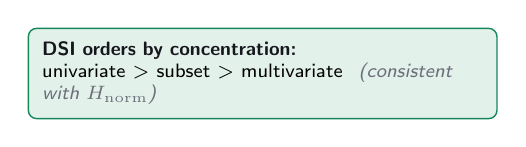
\begin{tikzpicture}[font=\scriptsize]
\node[fill=emerald!12,draw=emerald,line width=0.5pt,rounded corners=3pt,
      inner sep=5pt,text width=5.6cm,align=left] {%
\textbf{\color{ink}DSI orders by concentration:}\\
univariate $>$ subset $>$ multivariate
\;{\scriptsize\color{graphite}\itshape\,(consistent with $H_{\mathrm{norm}}$)}};
\end{tikzpicture}
\end{columns}
\end{frame}

% ──────────────────── RESULT 4 ────────────────────
\setsec{03 \textbar{} RESULT 4}
\begin{frame}{False-alarm robustness on stable streams}
\centering
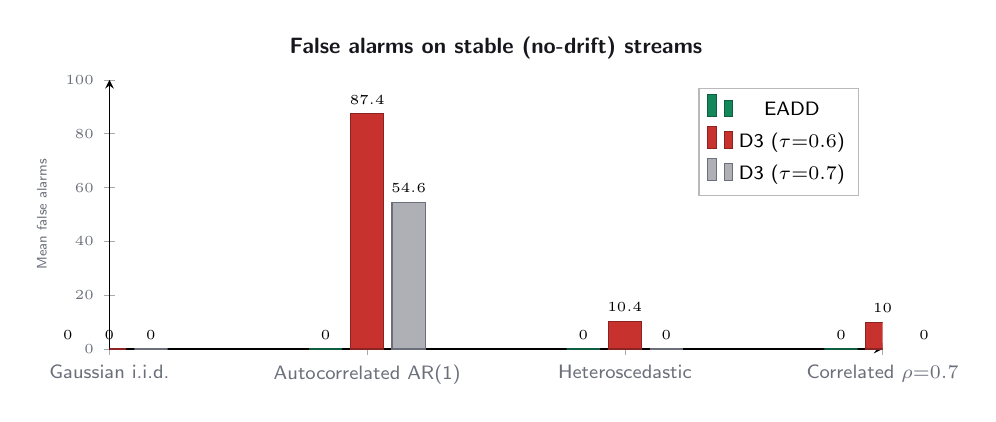
\begin{tikzpicture}[font=\tiny]
  \begin{axis}[
    width=11.4cm,height=5.0cm,
    title={\footnotesize\color{ink}\textbf{False alarms on stable (no-drift) streams}},
    title style={yshift=-2pt},
    ybar=3pt,bar width=12pt, ymin=0,ymax=100,
    enlarge x limits=0.20,
    symbolic x coords={Gaussian i.i.d.,Autocorrelated AR(1),Heteroscedastic,{Correlated $\rho{=}0.7$}},
    xtick=data,
    xticklabel style={font=\scriptsize,text=graphite,align=center},
    ylabel={Mean false alarms},
    axis lines=left,
    every axis label/.style={font=\tiny,text=graphite},
    every tick label/.style={font=\tiny,text=graphite},
    tick style={graphite!60}, every axis line/.style={graphite!60},
    nodes near coords, nodes near coords style={font=\tiny\bfseries},
    legend style={at={(0.97,0.97)},anchor=north east,legend columns=1,
                  font=\scriptsize,draw=ink!30,fill=white},
  ]
    \addplot[fill=emerald,draw=emerald!70!black]
      coordinates {(Gaussian i.i.d.,0) (Autocorrelated AR(1),0) (Heteroscedastic,0) ({Correlated $\rho{=}0.7$},0)};
    \addplot[fill=crimson,draw=crimson!70!black]
      coordinates {(Gaussian i.i.d.,0) (Autocorrelated AR(1),87.4) (Heteroscedastic,10.4) ({Correlated $\rho{=}0.7$},10.0)};
    \addplot[fill=graphite!55,draw=graphite]
      coordinates {(Gaussian i.i.d.,0) (Autocorrelated AR(1),54.6) (Heteroscedastic,0) ({Correlated $\rho{=}0.7$},0)};
    \legend{EADD,D3 ($\tau{=}0.6$),D3 ($\tau{=}0.7$)}
  \end{axis}
\end{tikzpicture}

\vspace{0.2em}
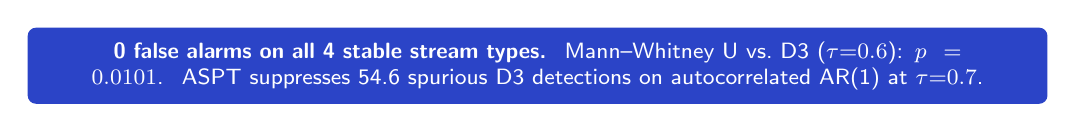
\begin{tikzpicture}[font=\footnotesize]
  \node[fill=cobalt,rounded corners=3pt,text=white,inner sep=5pt,
        text width=12.6cm,align=center] {%
    \textbf{0 false alarms on all 4 stable stream types.}\;
    Mann--Whitney U vs.\ D3 ($\tau{=}0.6$): \textbf{$p=0.0101$}.\;
    ASPT suppresses 54.6 spurious D3 detections on autocorrelated AR(1) at $\tau{=}0.7$.};
\end{tikzpicture}
\end{frame}

% ════════════════════ SECTION 4 ════════════════════
\sectionDivider{04}{Ablation \& Cost}{Where does the gain come from?}

\setsec{04 \textbar{} ABLATION}
\begin{frame}{Where does the gain come from?}
\begin{columns}[T,onlytextwidth]
\column{0.55\textwidth}
\centering
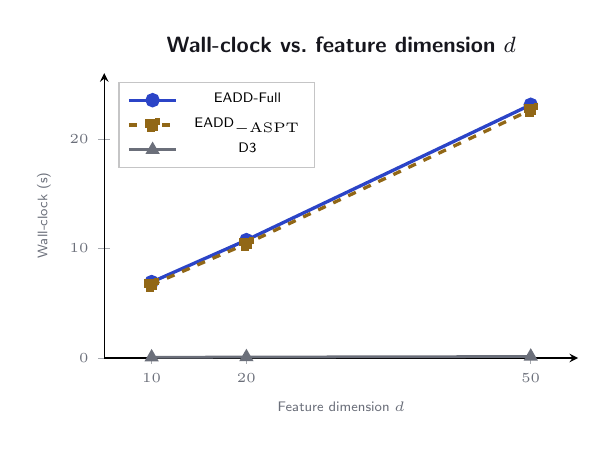
\begin{tikzpicture}[font=\tiny]
  \begin{axis}[
    width=7.6cm,height=5.2cm,
    title={\footnotesize\color{ink}\textbf{Wall-clock vs.\ feature dimension $d$}},
    title style={yshift=-2pt},
    xlabel={Feature dimension $d$}, ylabel={Wall-clock (s)},
    xmin=5,xmax=55,ymin=0,ymax=26,
    xtick={10,20,50},
    axis lines=left,
    every axis label/.style={font=\tiny,text=graphite},
    every tick label/.style={font=\tiny,text=graphite},
    tick style={graphite!60}, every axis line/.style={graphite!60},
    legend style={at={(0.03,0.97)},anchor=north west,font=\tiny,
                  draw=ink!25,fill=white,column sep=4pt},
    mark size=2pt,
  ]
    \addplot[cobalt,line width=1.2pt,mark=*]
      coordinates {(10,6.93) (20,10.76) (50,23.11)};
    \addplot[gold!75!black,line width=1.2pt,mark=square*,dashed]
      coordinates {(10,6.68) (20,10.43) (50,22.64)};
    \addplot[graphite,line width=1.0pt,mark=triangle*]
      coordinates {(10,0.07) (20,0.09) (50,0.14)};
    \legend{EADD-Full,EADD$_{-\mathrm{ASPT}}$,D3}
  \end{axis}
\end{tikzpicture}

\column{0.45\textwidth}
\vspace{0.4em}
\textbf{\color{ink}Decomposing the gain}

\smallskip
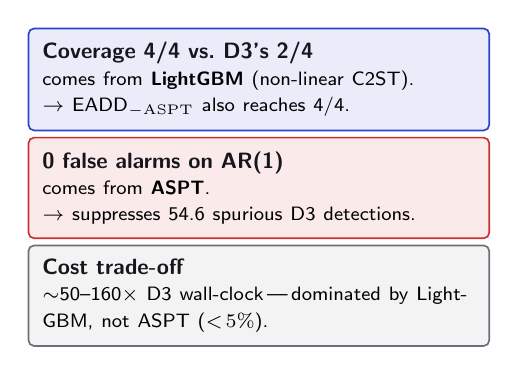
\begin{tikzpicture}[font=\footnotesize,
  card/.style={draw,line width=0.6pt,rounded corners=2pt,
               text width=5.5cm,align=left,inner sep=5pt}]
  \node[card,draw=cobalt,fill=cobalt!10] (a) {%
    \textbf{\color{ink}Coverage 4/4 vs.\ D3's 2/4}\\
    {\scriptsize comes from \textbf{LightGBM} (non-linear C2ST).}\\
    {\scriptsize $\to$ EADD$_{-\mathrm{ASPT}}$ also reaches 4/4.}};
  \node[card,draw=crimson,fill=crimson!10,below=2pt of a] (b) {%
    \textbf{\color{ink}0 false alarms on AR(1)}\\
    {\scriptsize comes from \textbf{ASPT}.}\\
    {\scriptsize $\to$ suppresses 54.6 spurious D3 detections.}};
  \node[card,draw=graphite,fill=graphite!8,below=2pt of b] (c) {%
    \textbf{\color{ink}Cost trade-off}\\
    {\scriptsize $\sim$50--160$\times$ D3 wall-clock\,---\,dominated by LightGBM, not ASPT ($<\!5\%$).}};
\end{tikzpicture}
\end{columns}
\end{frame}

% ════════════════════ SECTION 5 ════════════════════
\sectionDivider{05}{Limits \& Outlook}{What EADD cannot answer\,---\,yet}

\setsec{05 \textbar{} LIMITS}
\begin{frame}{Limitations \& future work}
\begin{columns}[T,onlytextwidth]
\column{0.50\textwidth}
\textbf{\color{crimson}Limitations}
\begin{itemize}\setlength\itemsep{2pt}\footnotesize
  \item Wall-clock $\sim$50--160$\times$ D3\,---\,LightGBM retrains every $M{=}50$ steps.
  \item \textbf{Multiple testing over time:} $\sim$600 tests/30K samples;
        Bonferroni $\alpha'{\approx}8.3{\times}10^{-5}$ below ASPT's $1/(B_{\max}{+}1){=}0.005$ floor.\\
        {\scriptsize\itshape Zero-FA result empirical, not theoretically guaranteed.}
  \item DSI tier boundaries heuristic; never triggered above LOW in experiments.
  \item SHAP attributions correlational, not causal.
  \item No isolation of reservoir sampling vs.\ window config contributions.
\end{itemize}

\column{0.50\textwidth}
\textbf{\color{emerald}Future work}
\begin{itemize}\setlength\itemsep{2pt}\footnotesize
  \item Anytime-valid \textbf{e-values} for streaming FWER control.
  \item \textbf{Causal} attribution (Budhathoki+ AISTATS 2021).
  \item Multi-domain \textbf{DSI calibration} to ground tier boundaries empirically.
  \item Adversarial robustness of discriminative drift detectors.
  \item Per-feature operating curves under correlation $\to$ feature-group SHAP.
\end{itemize}

\vspace{0.4em}

\begin{tikzpicture}[font=\scriptsize]
  \node[fill=ink,rounded corners=3pt,text=white,inner sep=6pt,
        text width=6.2cm,align=center,font=\scriptsize] {%
    \textbf{Open invitation.} EADD is a starting point\,---\,each gap above is a separate research thread.};
\end{tikzpicture}
\end{columns}
\end{frame}

% ════════════════════ CONCLUSION ════════════════════
\setsec{CONCLUSION}
\begin{frame}{Conclusion}
\vspace{0.3em}
\centering

\begin{tikzpicture}[font=\footnotesize,
    pill/.style={fill=ink,text=white,rounded corners=10pt,
                 inner xsep=12pt,inner ysep=6pt,font=\bfseries}]
  \node[pill] {EADD answers \textcolor{gold}{WHETHER},
               \textcolor{gold}{WHEN},
               \textcolor{gold}{WHICH}, and
               \textcolor{gold}{HOW SEVERE}\,---\,in one pipeline.};
\end{tikzpicture}

\vspace{0.8em}
\centering
\statTile{4/4}{coverage}{cobalt}\hfill
\statTile{0}{false alarms}{emerald}\hfill
\statTile{8$\boldsymbol{\times}$}{faster MTD}{crimson}\hfill
\statTile{1.00}{SHAP P@k}{gold!75!black}

\vspace{0.8em}
\begin{columns}[T,onlytextwidth]
\column{0.50\textwidth}
\textbf{\color{ink}What we built}
\begin{itemize}\setlength\itemsep{1pt}\footnotesize
  \item ASPT $+$ $H_{\mathrm{pred}}$\,---\,rigorous confirmation, 90--95\% perm savings.
  \item SHAP $+$ DSI\,---\,feature-level diagnosis $+$ severity.
  \item Benchmark vs.\ 7 unsupervised detectors.
\end{itemize}

\column{0.50\textwidth}
\textbf{\color{ink}What it gives MLOps}
\begin{itemize}\setlength\itemsep{1pt}\footnotesize
  \item Reliable alarms on autocorrelated production streams.
  \item Actionable diagnoses, not just binary flags.
  \item Severity-tiered prescriptions for response.
\end{itemize}
\end{columns}
\end{frame}

% ════════════════════ THANK YOU ════════════════════
\begin{frame}[plain,noframenumbering]

\begin{tikzpicture}[remember picture,overlay]
  \fill[ink] (current page.south west) rectangle (current page.north east);
  \fill[cobalt,opacity=0.55]
    (current page.south east) -- ([xshift=-7.5cm]current page.south east)
    -- ([xshift=-3.5cm]current page.north east) -- (current page.north east) -- cycle;
  \foreach \i in {0,1,2,3,4}{
    \draw[gold,opacity={0.12+0.03*\i},line width=0.6pt]
      ([xshift=2cm+0.4*\i cm,yshift=2cm+0.3*\i cm]current page.south west)
      circle ({1.0cm+0.4*\i cm});
  }
  \node[anchor=center,text=white,font=\fontsize{56}{60}\bfseries]
    at ([yshift=0.8cm]current page.center) {Thank you.};
  \node[anchor=center,text=gold,font=\Large\itshape]
    at ([yshift=-0.5cm]current page.center) {Questions \& discussion welcome.};
  \node[anchor=center,text=white,font=\small]
    at ([yshift=-1.8cm]current page.center)
    {\textbf{Nusrat Begum} \textbar{} \texttt{nusrat.beg@student.mahidol.ac.th}};
  \node[anchor=south,text=white!60,font=\scriptsize]
    at ([yshift=0.6cm]current page.south) {Code + paper available at the project repository.};
\end{tikzpicture}
\end{frame}

% ════════════════════ APPENDIX ════════════════════
\appendix
\setsec{APPENDIX}

\begin{frame}{Backup \textbar{} runtime scaling vs.\ window size $N_\mathrm{cur}$}
\begin{columns}[T,onlytextwidth]
\column{0.58\textwidth}
\centering
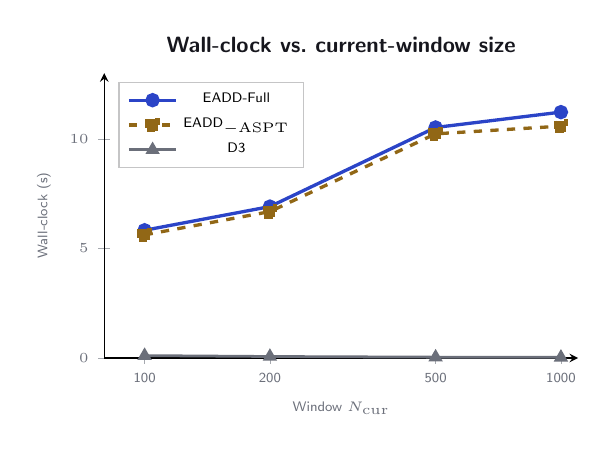
\begin{tikzpicture}[font=\tiny]
  \begin{axis}[
    width=7.6cm,height=5.2cm,
    title={\footnotesize\color{ink}\textbf{Wall-clock vs.\ current-window size}},
    title style={yshift=-2pt},
    xlabel={Window $N_\mathrm{cur}$}, ylabel={Wall-clock (s)},
    xmin=80,xmax=1100,ymin=0,ymax=13,
    xmode=log,log basis x=10,
    xtick={100,200,500,1000}, xticklabels={100,200,500,1000},
    axis lines=left,
    every axis label/.style={font=\tiny,text=graphite},
    every tick label/.style={font=\tiny,text=graphite},
    tick style={graphite!60}, every axis line/.style={graphite!60},
    legend style={at={(0.03,0.97)},anchor=north west,font=\tiny,
                  draw=ink!25,fill=white},
    mark size=2pt,
  ]
    \addplot[cobalt,line width=1.2pt,mark=*]
      coordinates {(100,5.83) (200,6.91) (500,10.52) (1000,11.22)};
    \addplot[gold!75!black,line width=1.2pt,mark=square*,dashed]
      coordinates {(100,5.62) (200,6.68) (500,10.23) (1000,10.58)};
    \addplot[graphite,line width=1.0pt,mark=triangle*]
      coordinates {(100,0.11) (200,0.07) (500,0.04) (1000,0.03)};
    \legend{EADD-Full,EADD$_{-\mathrm{ASPT}}$,D3}
  \end{axis}
\end{tikzpicture}

\column{0.42\textwidth}
\vspace{0.6em}
\begin{itemize}\footnotesize\setlength\itemsep{3pt}
  \item $N_\mathrm{cur}{=}200{\to}1000$: EADD time grows only \textbf{1.6$\times$}.
  \item LightGBM cost sub-linear in $N$, near-linear in $d$.
  \item ASPT overhead $<\!5\%$ across window sizes.
\end{itemize}

\vspace{0.5em}
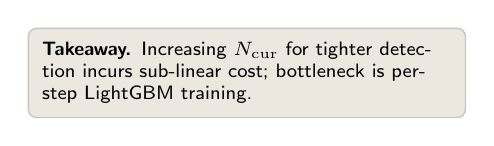
\begin{tikzpicture}[font=\footnotesize]
  \node[fill=mist,draw=ink!25,line width=0.5pt,rounded corners=3pt,
        inner sep=5pt,text width=5.2cm,align=left,font=\scriptsize] {%
    \textbf{Takeaway.} Increasing $N_\mathrm{cur}$ for tighter detection incurs sub-linear cost;
    bottleneck is per-step LightGBM training.};
\end{tikzpicture}
\end{columns}
\end{frame}

\begin{frame}{Backup \textbar{} correlated features ($d{=}10$)}
\begin{columns}[T,onlytextwidth]
\column{0.55\textwidth}
\centering
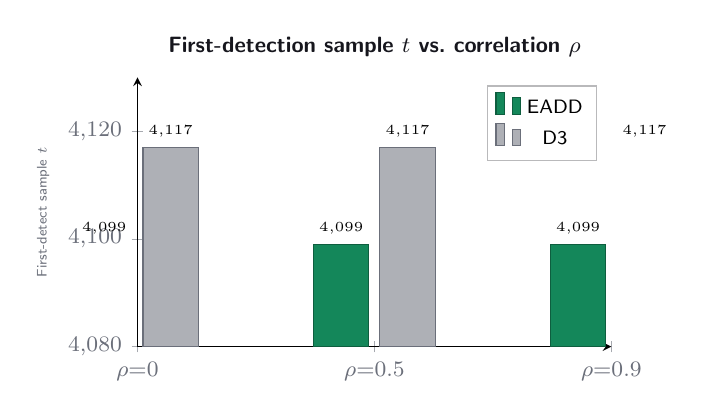
\begin{tikzpicture}[font=\tiny]
  \begin{axis}[
    width=7.6cm,height=5.0cm,
    title={\footnotesize\color{ink}\textbf{First-detection sample $t$ vs.\ correlation $\rho$}},
    title style={yshift=-2pt},
    ybar=4pt,bar width=20pt, ymin=4080,ymax=4130,
    enlarge x limits=0.25,
    symbolic x coords={$\rho{=}0$,$\rho{=}0.5$,$\rho{=}0.9$},
    xtick=data, ylabel={First-detect sample $t$},
    axis lines=left,
    every axis label/.style={font=\tiny,text=graphite},
    every tick label/.style={font=\footnotesize,text=graphite},
    tick style={graphite!60}, every axis line/.style={graphite!60},
    nodes near coords, nodes near coords style={font=\tiny\bfseries},
    legend style={at={(0.97,0.97)},anchor=north east,legend columns=1,
                  font=\scriptsize,draw=ink!30,fill=white},
  ]
    \addplot[fill=emerald,draw=emerald!70!black]
      coordinates {($\rho{=}0$,4099) ($\rho{=}0.5$,4099) ($\rho{=}0.9$,4099)};
    \addplot[fill=graphite!55,draw=graphite]
      coordinates {($\rho{=}0$,4117) ($\rho{=}0.5$,4117) ($\rho{=}0.9$,4117)};
    \legend{EADD,D3}
  \end{axis}
\end{tikzpicture}

\column{0.45\textwidth}
\vspace{0.8em}
\begin{itemize}\footnotesize\setlength\itemsep{4pt}
  \item Cholesky-mixed Gaussian; $+2\sigma$ shift in 3 features at $t{=}4000$.
  \item EADD detection robust to correlation; stable correlated streams give \textbf{0 FA}.
  \item SHAP under correlation $\to$ interpret at \textbf{feature-group} granularity.
\end{itemize}
\end{columns}
\end{frame}

\end{document}
